\clearpage
\onecolumn
\appendix
\section{Семейственные профили}
\begin{figure}[!ht]
\centering
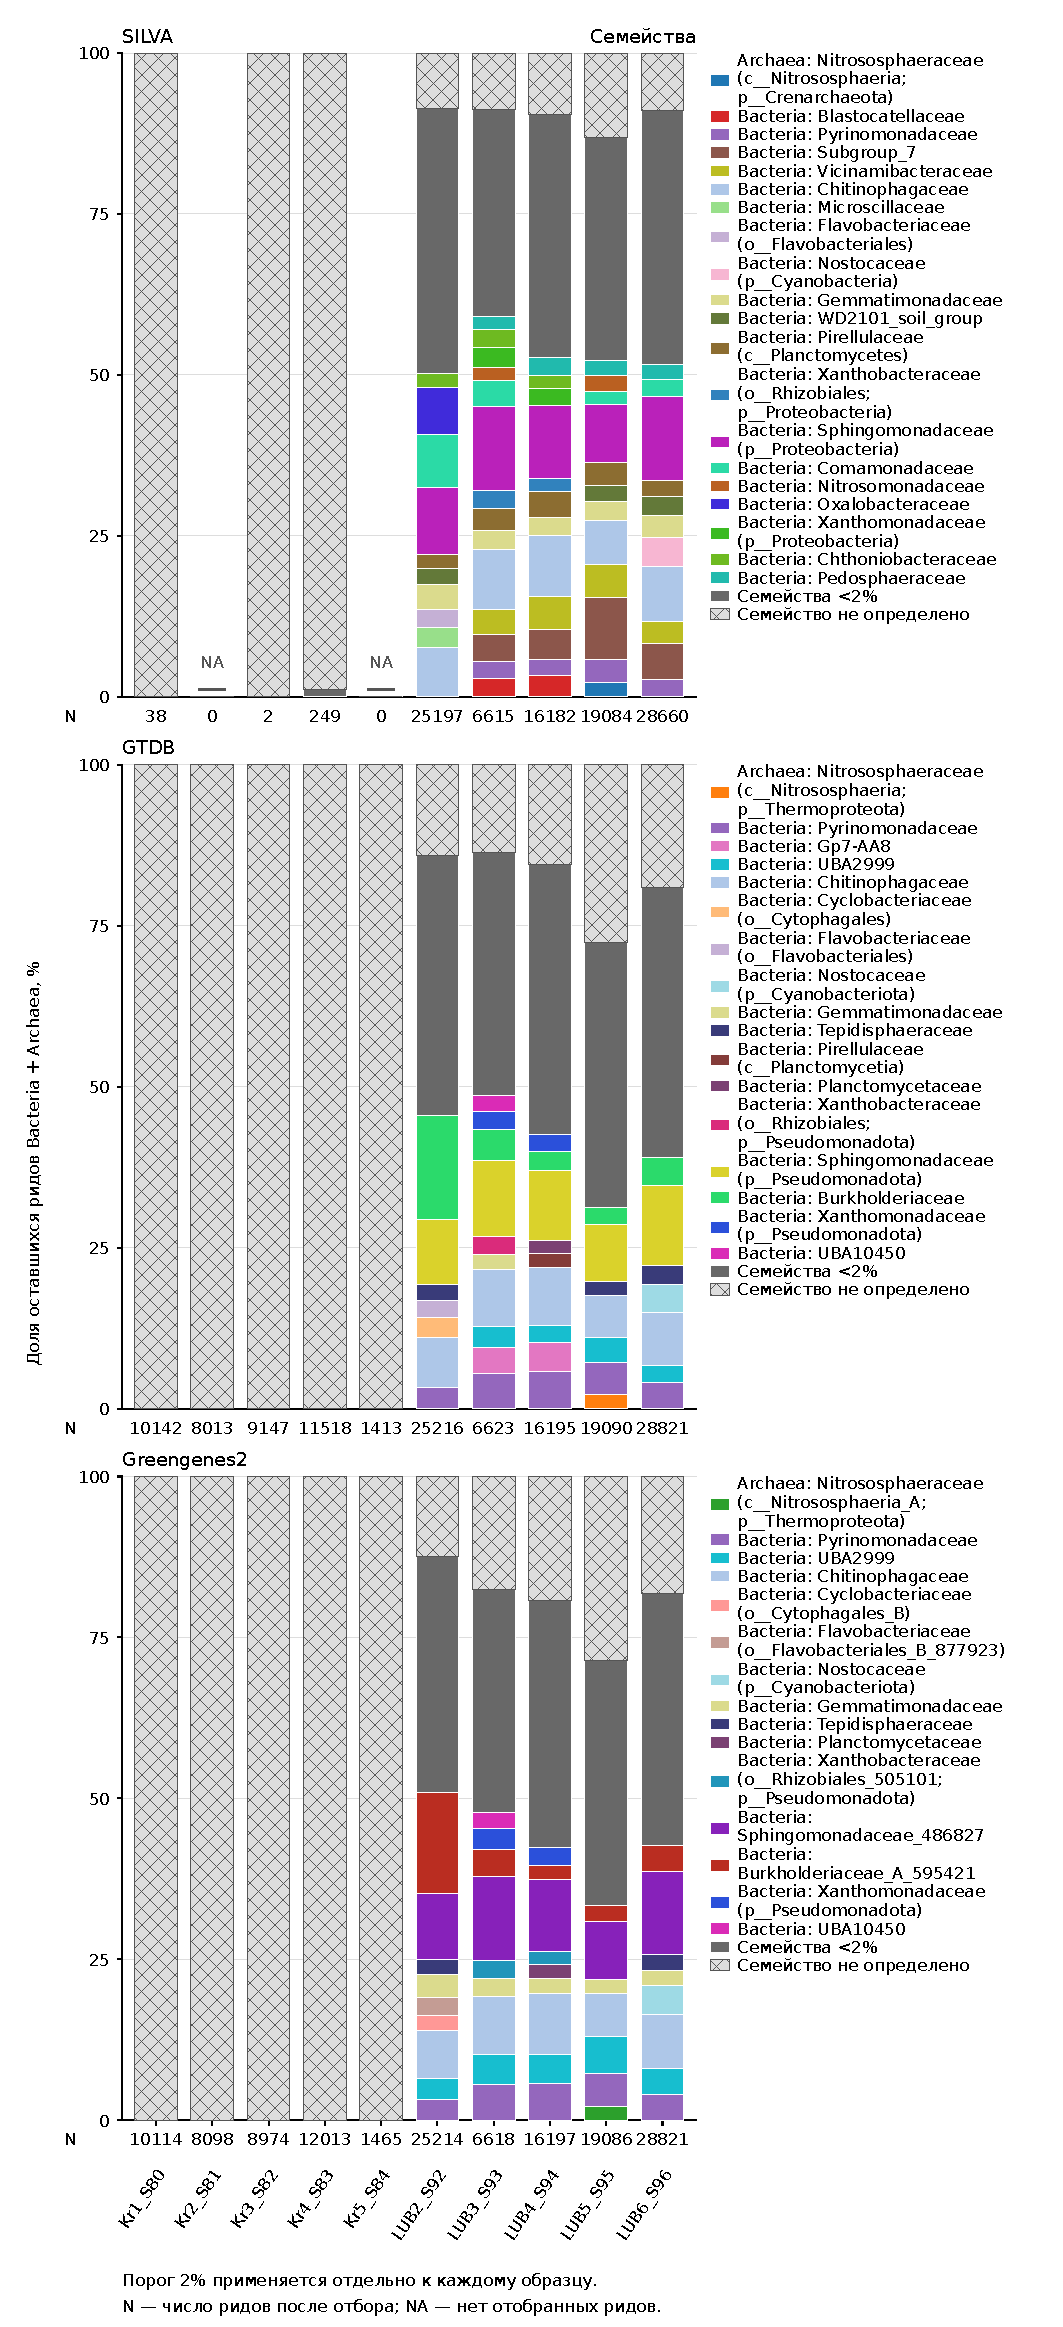
\includegraphics[width=\textwidth,trim=0bp 766.03bp 0bp 0bp,clip]{../../figures/taxonomy/family/prokaryotic_family_overview.pdf}
\caption{\porozhdeno{\Claim{F01}{Обзор, верхняя панель: SILVA. Показаны почвы, контроль исключён. Отбор Bacteria + Archaea исключает явные органелльные метки; $N$ зависит от модели. Неопределённое семейство (\texttt{UNCLASSIFIED}, включая точное \texttt{f\_\_uncultured}) остаётся в $N$ и показано штриховкой; при $N=0$ --- NA. Серым объединены назначенные семейства ниже \SelectedDisplayThresholdPct{}\% данного образца без удаления ридов. Обзор разделён на смежные полосы для читаемости; порядок образцов общий и подписан на нижней панели.}}}
\label{fig:overview}
\end{figure}
\clearpage
\begin{figure}[!ht]
\ContinuedFloat
\centering
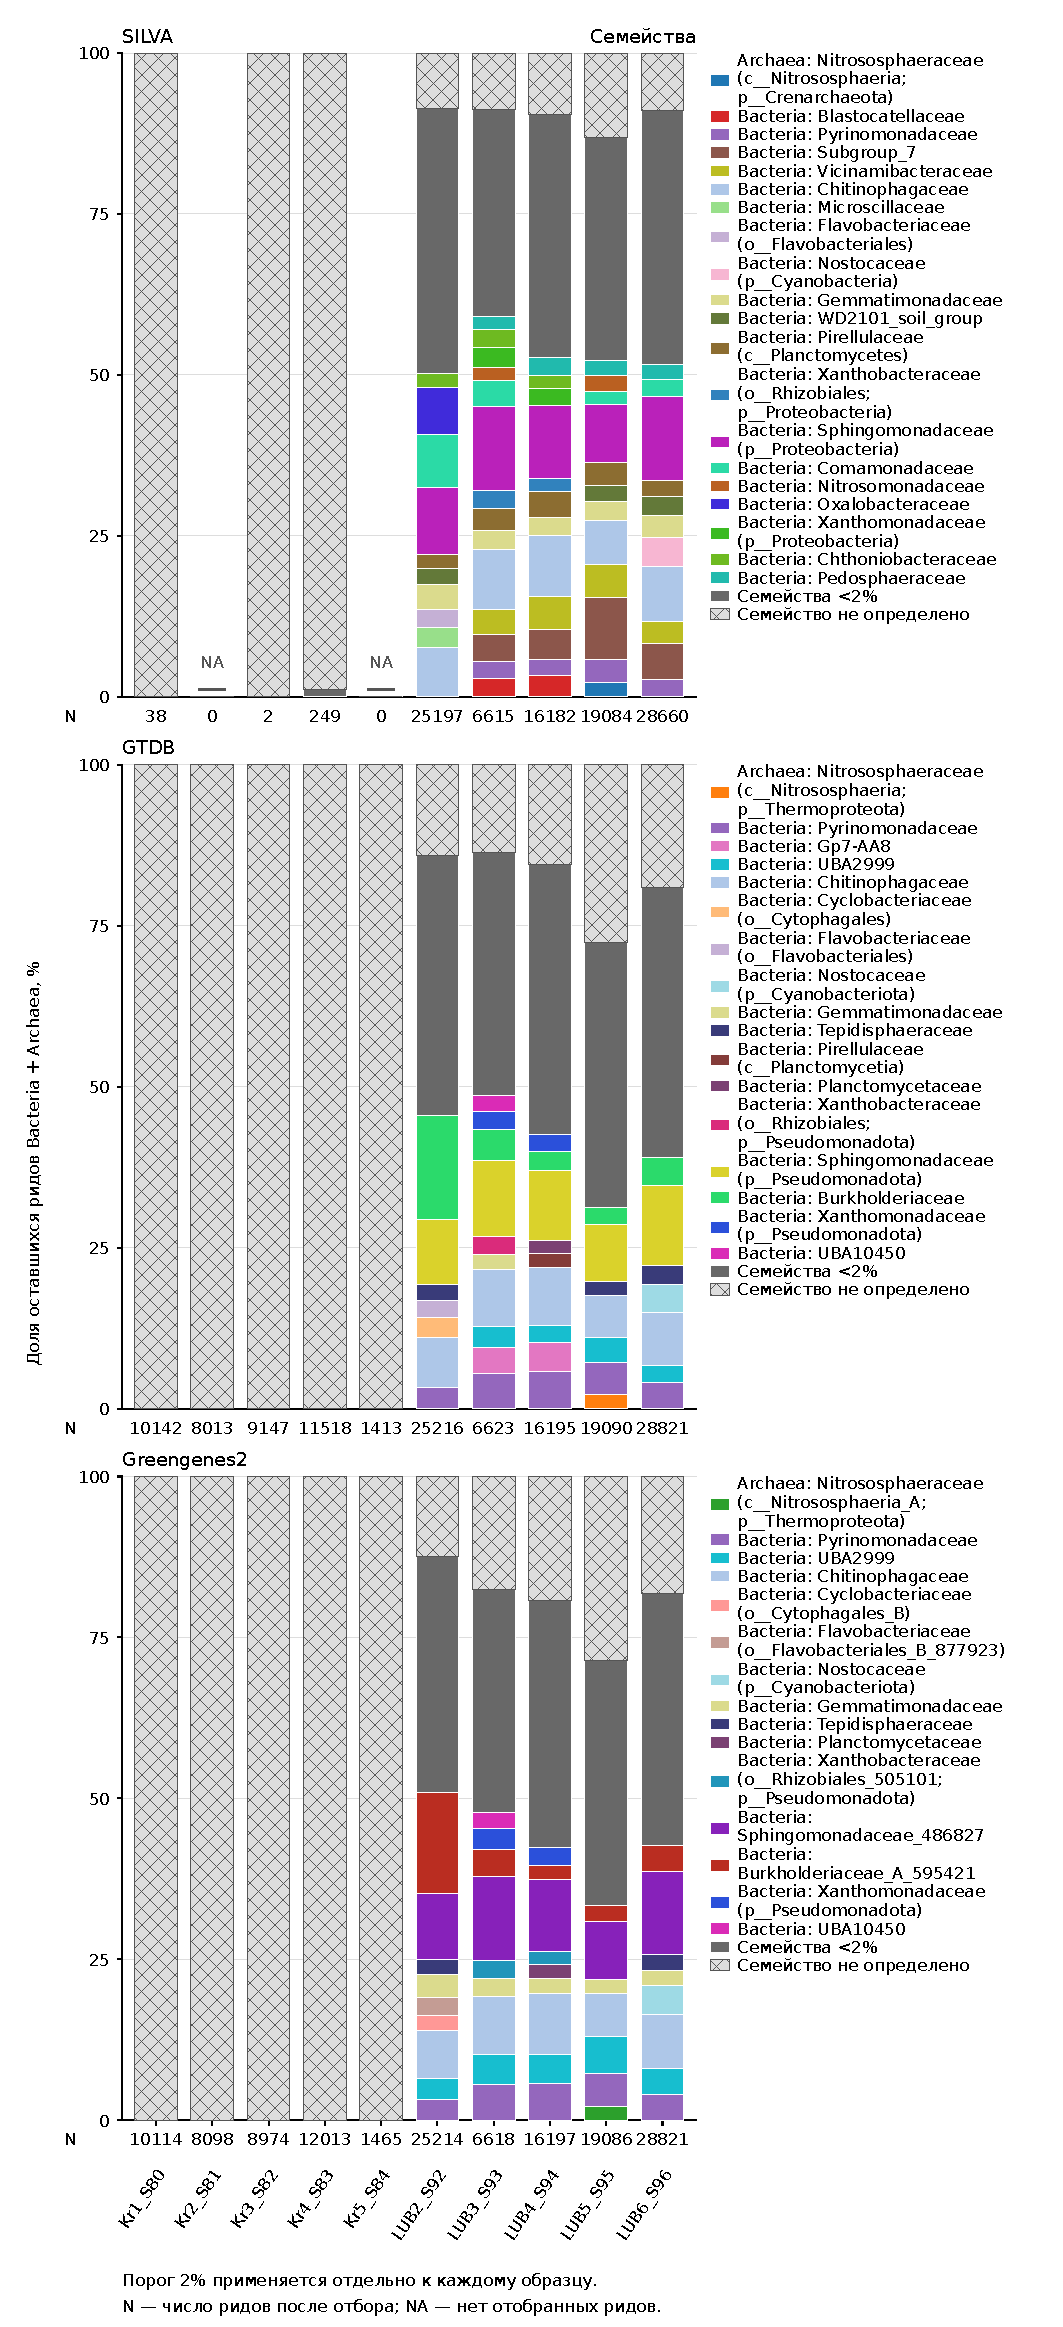
\includegraphics[width=\textwidth,trim=0bp 424.03bp 0bp 351bp,clip]{../../figures/taxonomy/family/prokaryotic_family_overview.pdf}
\caption{\porozhdeno{\Claim{F01B}{Продолжение обзора: GTDB. Знаменатель --- модельный $N$ после отбора Bacteria + Archaea и исключения явных органелльных меток; \texttt{UNCLASSIFIED} входит в $N$, пустой отбор обозначается NA. Порог объединения назначенных семейств --- \SelectedDisplayThresholdPct{}\% данного образца. Цвета и названия относятся к легенде этой модели; совпадение цвета между моделями не является сопоставлением таксонов.}}}
\label{fig:overviewmiddle}
\end{figure}
\clearpage
\begin{figure}[!ht]
\ContinuedFloat
\centering
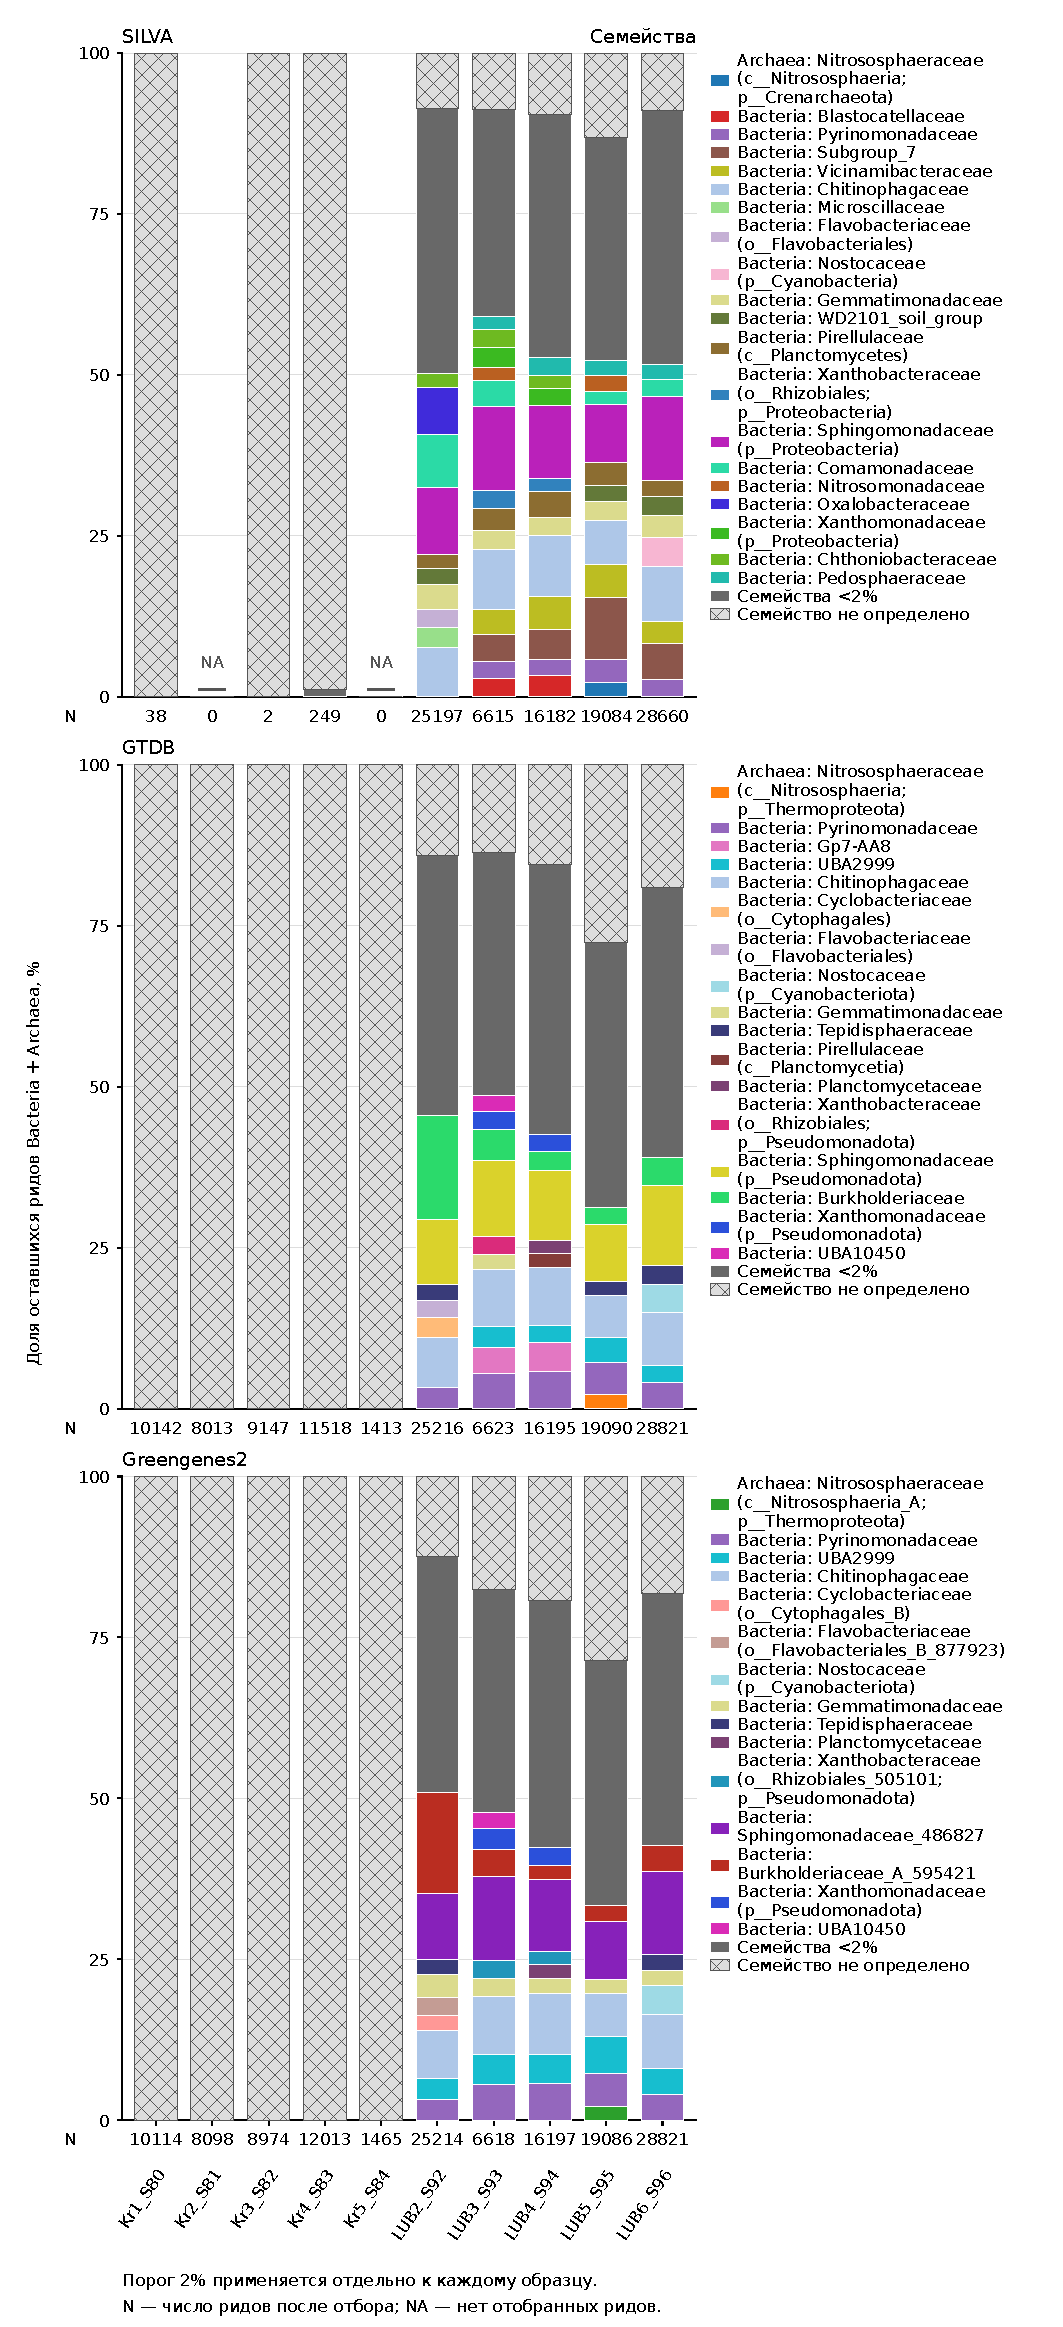
\includegraphics[width=\textwidth,trim=0bp 0bp 0bp 693bp,clip]{../../figures/taxonomy/family/prokaryotic_family_overview.pdf}
\caption{\porozhdeno{\Claim{F01C}{Окончание обзора: GG2 и общий порядок почвенных образцов. Знаменатель --- $N$ после модельного отбора Bacteria + Archaea без явных органелльных меток. \texttt{UNCLASSIFIED} остаётся в $N$, при $N=0$ --- NA; назначенные семейства ниже \SelectedDisplayThresholdPct{}\% объединены серым. Это нижняя смежная полоса того же исходного рисунка.}}}
\label{fig:overviewbottom}
\end{figure}
\clearpage
\begin{figure}[!ht]
\centering
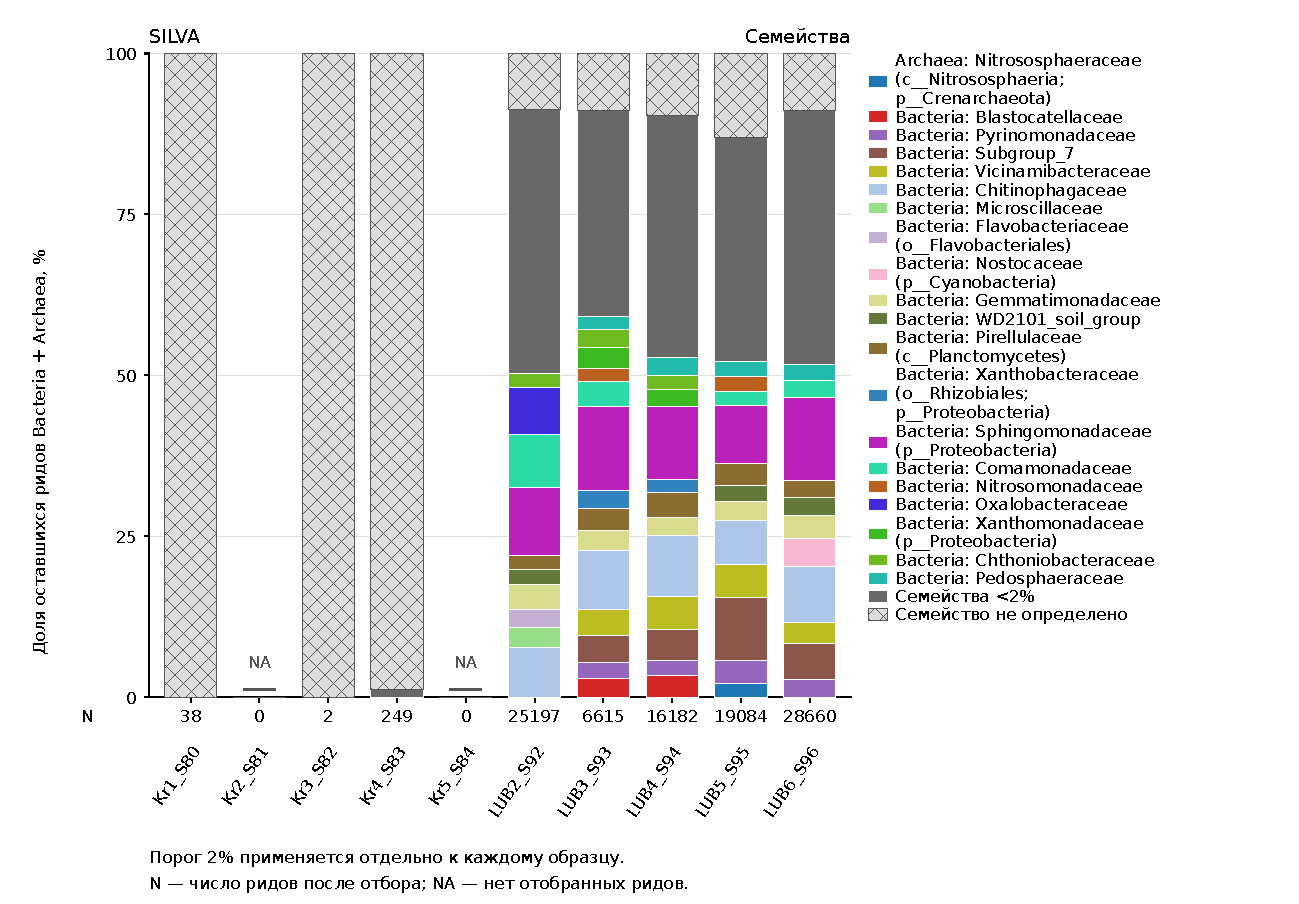
\includegraphics[width=\textwidth]{../../figures/taxonomy/family/prokaryotic_family_silva.pdf}
\caption{\porozhdeno{\Claim{F02}{Подробный профиль SILVA. Почвы после модельного отбора Bacteria + Archaea и исключения явно помеченных органелл; знаменатель каждого столбца --- его $N$. \texttt{UNCLASSIFIED} остаётся в знаменателе, точное \texttt{f\_\_uncultured} отнесено к нему; $N=0$ даёт NA. Семейства ниже \SelectedDisplayThresholdPct{}\% данного образца объединены без удаления ридов. Контроль не изображён.}}}
\label{fig:silva}
\end{figure}
\clearpage
\begin{figure}[!ht]
\centering
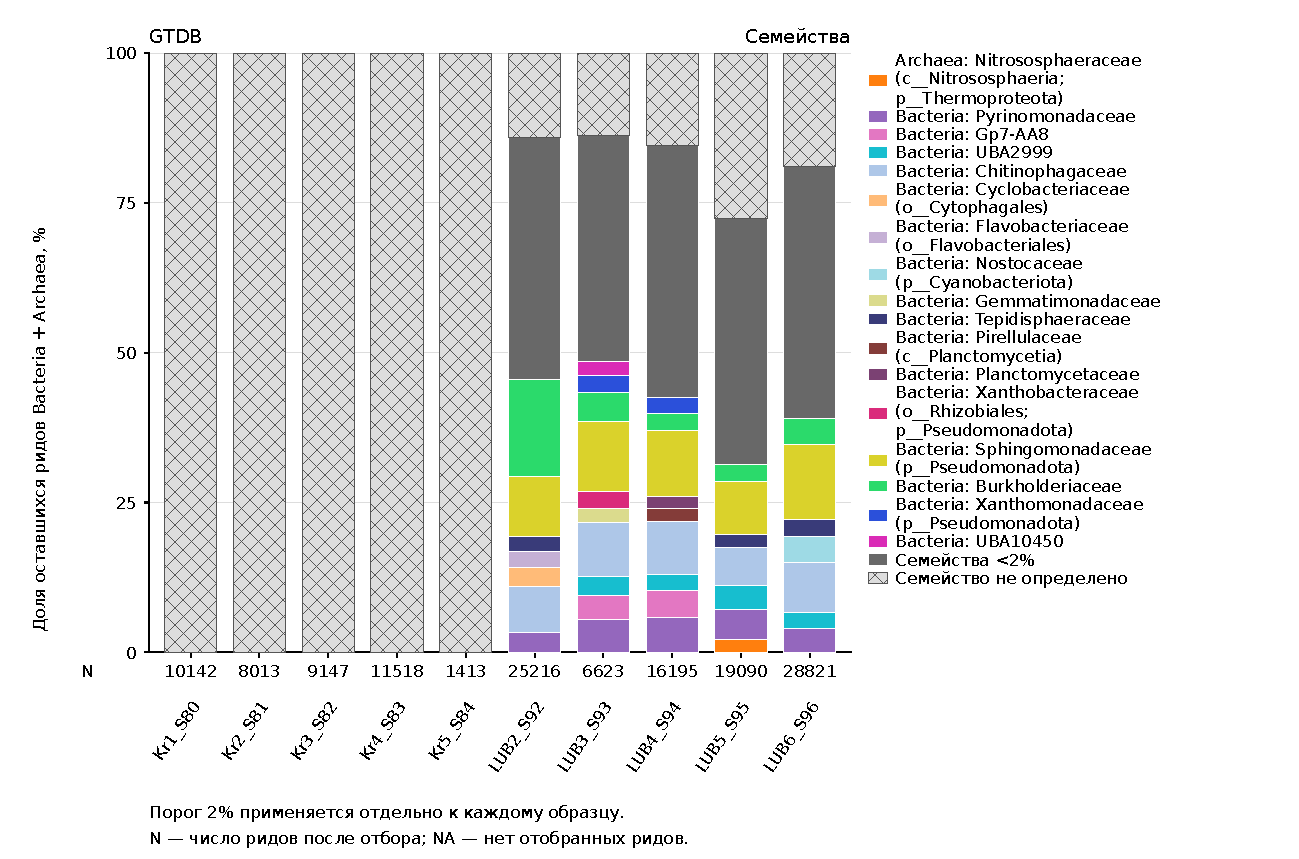
\includegraphics[width=\textwidth]{../../figures/taxonomy/family/prokaryotic_family_gtdb.pdf}
\caption{\porozhdeno{\Claim{F03}{Подробный профиль GTDB. Почвы после модельного отбора Bacteria + Archaea и исключения явно помеченных органелл; знаменатель --- собственный $N$ модели. \texttt{UNCLASSIFIED} включает неопределённые семейства и точное \texttt{f\_\_uncultured}; при $N=0$ доля была бы NA. Назначенные семейства ниже \SelectedDisplayThresholdPct{}\% сгруппированы без удаления ридов. Контроль исключён из рисунка.}}}
\label{fig:gtdb}
\end{figure}
\clearpage
\begin{figure}[!ht]
\centering
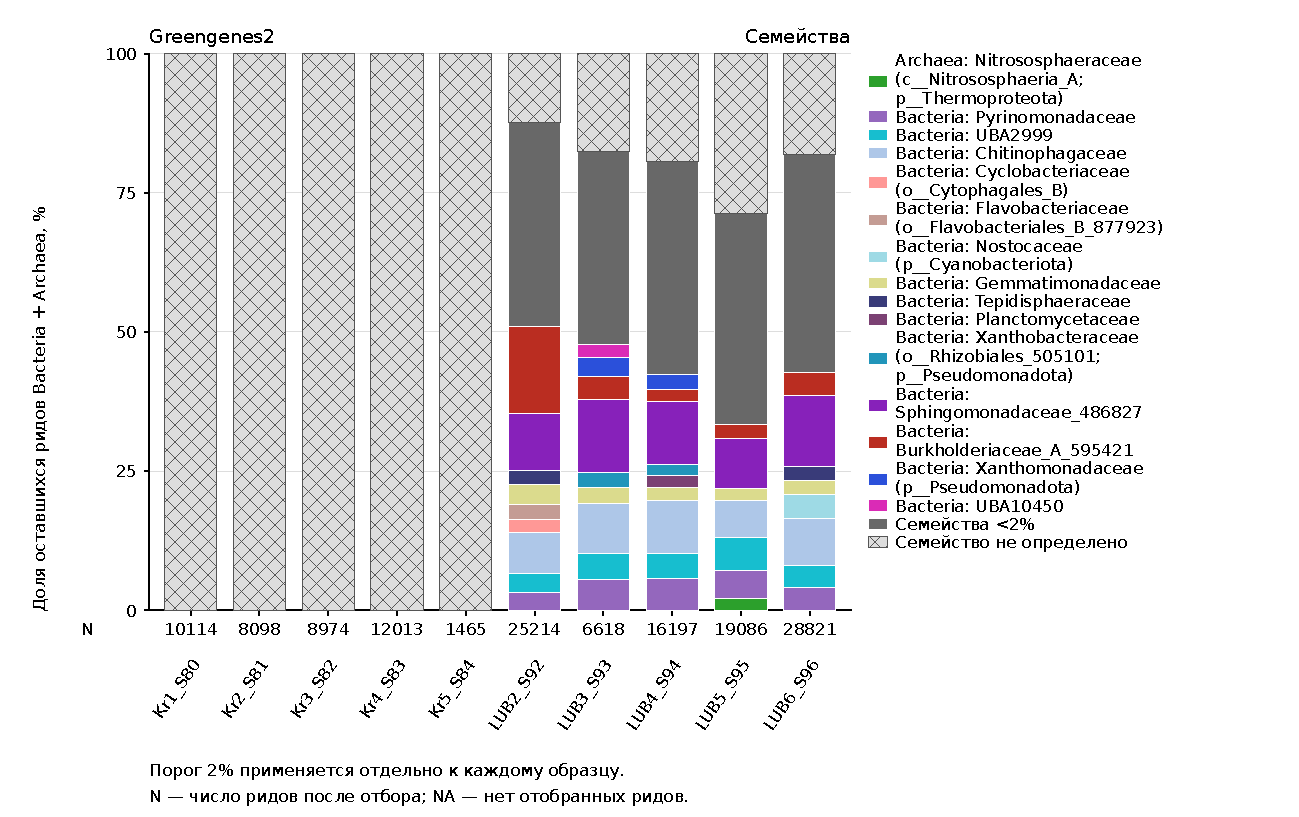
\includegraphics[width=\textwidth]{../../figures/taxonomy/family/prokaryotic_family_gg2.pdf}
\caption{\porozhdeno{\Claim{F04}{Подробный профиль GG2. Почвы после модельного отбора Bacteria + Archaea и исключения явно помеченных органелл; знаменатель --- собственный $N$ модели с сохранённым \texttt{UNCLASSIFIED}, включая точное \texttt{f\_\_uncultured}. Пустой отбор означал бы NA. Назначенные семейства ниже \SelectedDisplayThresholdPct{}\% объединены серым, их риды остаются в $N$. Контроль не изображён.}}}
\label{fig:ggtwo}
\end{figure}
